\chapter{Experimental Results}
\label{results}

\section{Introduction}

In this chapter the we examine four samples from around the University
(See Table~\ref{results:sampletable}), taken over a period of five
months during 1994.  The results are displayed as graphs along with
commentary about any notable features.  There are also notes on how
the graphs were obtained and any interesting results.

The samples have been taken from quite different environments to try
to give a wide selection of network protocols and traffic conditions.
Along with the results of the four samples, one of the samples has
been split up by network protocol.  The question of how each different
protocol affects the traffic behaviour is one this thesis would like
to try to answer, or at least gauge the basic similarities and
differences between the protocols.

\begin{table}
{\small \begin{tabular}{|l|l|l|l|l|l|} \hline
Date & Location & Traffic Mix & Load & Time & Packet Count \\ \hline \hline
14 May & Computer Centre & AppleTalk, Telnet & Heavy & 14 minutes & 400,021 \\
 & Staff Network & Novell client & & & \\ \hline
13 June & Gateway to & Various IP & Light & 102 minutes & 329,379 \\
 & Outside World & & & & \\ \hline 
1 August & Statistics & IP, mainly NFS & Light & 118 minutes & 400,048 \\
 & & & & & \\ \hline
1 September & Commerce & NetBIOS from & Medium & 94 minutes & 800,002 \\
 & & Windows NT & & & \\ \hline
\end{tabular}}
\caption{Traffic Samples from around The University of Auckland}
\label{results:sampletable}
\end{table}

\section{Processing trace files}

Once the trace file has been recorded it is transfered to a Unix host
where it is processed.  The first processing done corrects the timer
problem (Section~\ref{trace:timerprob}).  The file may then be divided
up, based on the various protocols embedded in the packet, and used to
generate packet frequency (by time interval) data.

\subsection{Correcting the timer problem}

The correcting of the timer problem is a simple process.  Because the
timer error causes a time to be out by 256, by keeping some notion of
the minimum correct time we can determine whether a time-stamp is
earlier than it should be.  Adding 256 to the value corrects the
time-stamp to the right value.  This is done by the program

{\ttfamily \small \begin{flushleft}
  correct filename[.icr]
\end{flushleft}}
which produces a new file called {\ttfamily {\em filename}.tra}.  {\ttfamily
correct} also changes the time from ticks ($\sim 4648$ ticks per
second) to milliseconds.  This greatly simplifies all calculations and
removes any dependence on the PC timers.

\subsection{Producing frequency data}

The process of producing discrete time interval packet and octet
counts is very simple.  The program {\ttfamily arrival} is given the slot
size in milliseconds and told whether the output should be a binary
file or an ASCII text file.

{\ttfamily \small \begin{flushleft}
  arrival [-b binary] [-t interval time] filename[.tra]
\end{flushleft}}

\begin{figure}[t]
\begin{center}
{\ttfamily
\begin{tabular}{ccc}
4649	& 65	& 11524 \\
4650	& 66	& 12652 \\
4651	& 61	& 12261 \\
4652	& 56	& 10319 \\
4653	& 54	& 12231 \\
4654	& 57	& 10219 \\
4655	& 58	& 10704 \\
4656	& 66	& 12109 \\
4657	& 49	& 10574 \\
4658	& 60	& 11231 \\
4659	& 49	& 10424 \\
\end{tabular}}
\end{center}
\caption{Sample output of {\em arrival}}
\label{interval:figure1}
\end{figure}

The text output of {\ttfamily arrival} can be seen in
Figure~\ref{interval:figure1}.  The first column is the interval
number, the second the packet count and the third the total number of
octets.  The binary output has the same format except that the entries
are stored as 32 bit integer values.  The binary file also has the
total number of rows and columns stored at the end of the file as 32
bit integer values.  This is to help programs which read the file.

\subsection{Dividing trace into protocols}

To provide information on individual protocols packet traces need to
be separated.  This is done by a program {\ttfamily demux} (for
demultiplex), which takes each packet header in turn, analyses it and
decides via a set of rules which output file to store it in.

Currently the rules provide for IP, AppleTalk, IPX and most of DECnet.
As IP, IPX and AppleTalk make up the bulk of all the University's
network traffic this is adequate.

\subsection{Producing the histograms}

The histograms (figures \ref{results:snet1.1s.hist},
\ref{results:snet93.1s.hist}, \ref{results:gatew.1s.hist}, \ldots) were
produced using the following program:

{\ttfamily \small \begin{flushleft} hist [-w width] [-s smooth] filename[.tra]
\end{flushleft}}

{\ttfamily hist} reads in the files created by {\ttfamily arrival} and produces a
frequency histogram table.  As the input is packets per time unit
(normally one second) this gives us an indication of how the traffic
levels are spread.  This table is stored as ASCII so it can be
directly plotted.  To get around the problem of too much detail an
aggregation (smoothing) feature was added.  This takes the histogram
results and at successive intervals of size $s$ it sums the frequency
values, and outputs a single value for the interval at the average of the
corresponding packets per second.

\subsection{Producing slowly decaying variance results}
\label{results:stat}

To produce the slowly decay variance results the output from {\ttfamily
arrival} has to be processed.  This is done using the program

{\ttfamily \small \begin{flushleft}
  stat [-l logarithmic output] [-v verbose] [-m maximum] filename[.abf] ... \\
\end{flushleft}}
which automatically detects whether the file is text or binary and
reads it all into memory.  From the input file it builds up a vector
$\vec{u}$ in memory containing all the packet count values, say $size$
long.  Let the command line maximum be stored as $cmdmax$.

It then loops from $1$ to $\mbox{min}(size / 100, cmdmax)$ using the
variable $k$.  Let 
\[
\vec{v}_{k} \mbox{ be vectors of length } k
\]
 such that
\[
\vec{v}_{k_l} = \sum^{k \cdot (l+1) - 1}_{i = k \cdot l}{\vec{u}_i} / k
\mbox{ where } l \in \{0, \ldots, size \mbox{ div } k - 1\} \subset{\mathbb N}
\]

Let $var_k$ be the sample variance of the vector $\vec{v}_k$.  The
output file {\ttfamily {\em filename}.sta} is the textual representation of
the ordered pairs $(k, var_k)$.  If the {\ttfamily -l} command flag is
present then another file called {\ttfamily {\em filename}.dat} is also
produced with the ordered pairs $(\log_{10} k, \log_{10} var_k)$.

\section{Mean and standard deviation of samples}

\begin{table}[t]
\begin{center}
{\begin{tabular}{|p{4cm}|r|r|r|} \hline
Sample & Interval & Mean & Std. Dev \\ \hline \hline
Gateway Network & 10s	& 537.50 &  115.33 \\
		& 1s    &  53.70 &   17.48 \\
		& 100ms &   5.37 &    3.39 \\
		& 10ms  &   0.53 &    0.86 \\ \hline
Computer Centre & 10s & 3,008.00 & 1405.31 \\
		& 1s  &   300.70 &  188.77 \\
		& 100ms &  30.08 &   23.37 \\
		& 10ms  &   3.01 &    2.99 \\ \hline
Statistics	& 10s &   561.00 &  426.23 \\
		& 1s  &    56.10 &   64.89 \\
		& 100ms &   5.61 &    9.13 \\
		& 10ms  &   0.56 &    1.43 \\ \hline
Commerce	& 10s & 1,408.50 &  559.17 \\
		& 1s  &   140.85 &   69.06 \\
		& 100ms &  14.08 &    9.05 \\
		& 10ms  &   1.41 &    1.70 \\ \hline 
\end{tabular}}
\end{center}
\caption{Mean and Variance of Samples}
\label{results:means}
\end{table}

Table~\ref{results:means} lists the means and standard deviations of
the samples with different aggregation times.  The aggregation can be
seen as a simple non-overlapping summation (\S
\ref{models:aggregation}).  The means increase linearly as expected due
to the linear nature of expectation.

Taking the 10 millisecond results as a starting point, if the
underlying model is a Poisson process then we would expect the
standard deviations to increase by a factor of order $\sqrt{10}$ each
step.  Instead we see they increase much faster, giving strength to
the argument that Ethernet traffic is non-Poisson in nature.

\section{Graphs of results}

Below are a collection of graphs showing packet count against time (figures 
\ref{results:snet1.1s.freq}, \ref{results:snet1.10ms.freq},
\ref{results:snet93.1s.freq}, \ref{results:snet93.10ms.freq},
\ref{results:gatew.1s.freq}, \ref{results:gatew.10ms.freq},
\ref{results:pgrad.1s.freq}, \ref{results:pgrad.10ms.freq}).
Although little statistical information can be gained from these
graphs the wide range of different behaviours exhibited by Ethernet
traffic is readily apparent.

An attempt was made to try and get a wide sample of different traffic
behaviours from around the university campus.  We start by examining
graphs of packet counts against time.

\subsection{Packet Count versus octet count}

The packet traces produce two sets of data, namely packet counts and
octet counts.  Because Ethernet packets can have from 64 to 1518 bytes
of data, octet counts and packets counts are not equatable quantities.

Packet sizes are not evenly distributed.  In general they have a
multi-modal distribution which is based on the underlying protocol
stacks.  Each protocol has a maximum packet size and packets will be
that size unless they are the last packet in a sequence.  For example,
AppleTalk has a maximum of 600 bytes of data and TCP normally uses
only 1024 bytes, whereas NFS and Netware will use all 1500 bytes if
possible.  Many of the packets are also acknowledgement packets which
are only about 20 bytes long and fixed in size.  IPX for example
requires an acknowledgement packet for every data packet.

It was decided that packet counts were to be used rather than octet
counts for simplicity.  In some newer transmission technologies the
packet size is fixed so the difference disappears, packets are padded
with zeros if there isn't enough data to fill them.  The use of packet
counts rather octet counts also makes comparisons with simulations
simpler.

When bursts of traffic occur it is normally because of large
transfers.  In this case a majority of the packets will be of maximum
size so we can assume fixed maximum sized packets (at least when
looking at bursts).  In these cases packet counts are equivalent to
octet counts.

From examing time series graphs and slowly decaying variance graphs
produced for both packet counts and octets counts it was decided that
their behaviour was similar enough that not using the octet count
results would not be a loss.

\subsection{Graphs by segment}

\subsubsection{University Computer Centre network}

\begin{figure}
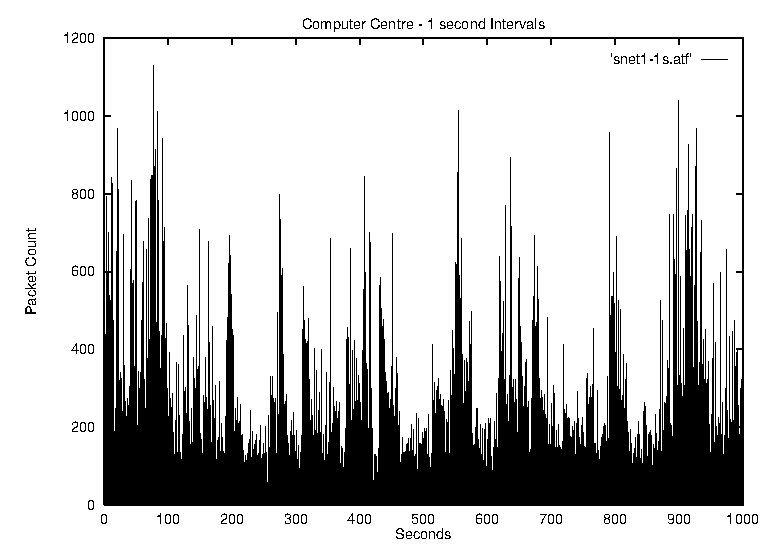
\includegraphics[height=3in]{pics/snet1-1s-freq.eps}
\caption{Computer Centre network with time interval 1 second}
\label{results:snet1.1s.freq}
\end{figure}

\begin{figure}
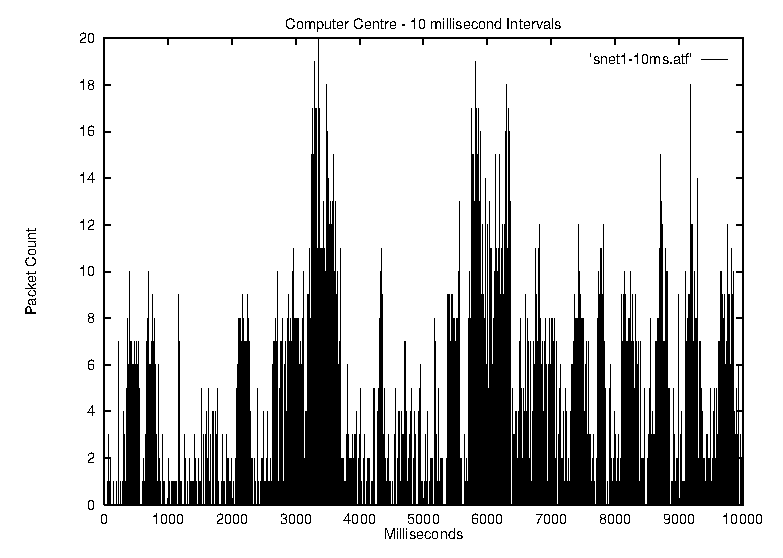
\includegraphics[height=3in]{pics/snet1-10ms-freq.eps}
\caption{Computer Centre network with time interval 10 milliseconds}
\label{results:snet1.10ms.freq}
\end{figure}

\begin{figure}
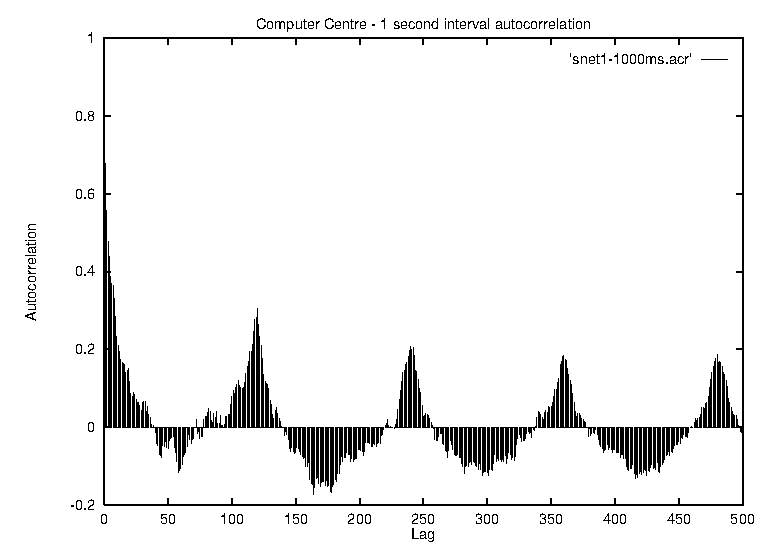
\includegraphics[height=3in]{pics/snet1-1s-acr.eps}
\caption{Computer Centre network autocorrelation with time interval 1 second}
\label{results:snet1.1s.acr}
\end{figure}

\begin{figure}
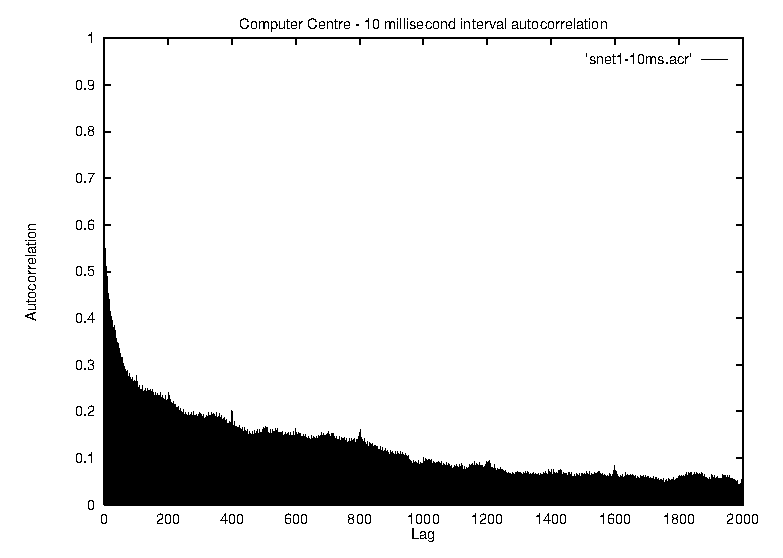
\includegraphics[height=3in]{pics/snet1-10ms-acr.eps}
\caption{Computer Centre network autocorrelation with time interval 10 milliseconds}
\label{results:snet1.10ms.acr}
\end{figure}

\begin{figure}
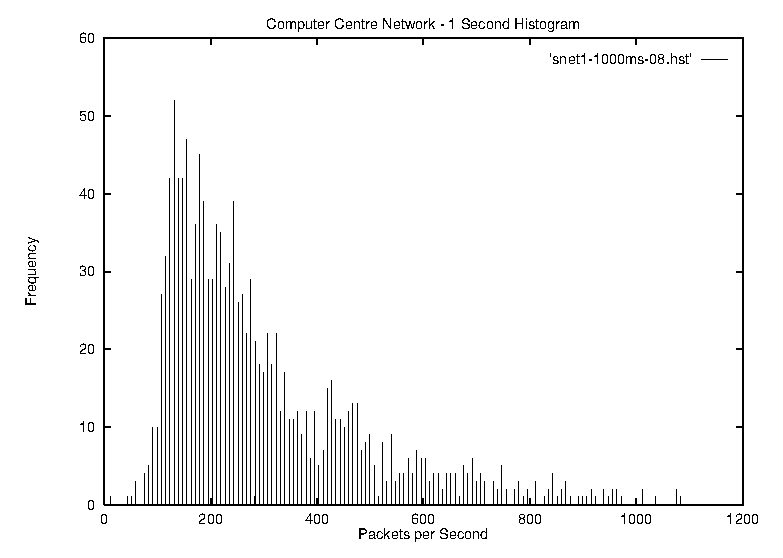
\includegraphics[height=3in]{pics/snet1-1s-hist-08.eps}
\caption{Computer Centre network histogram with time interval 1 second}
\label{results:snet1.1s.hist}
\end{figure}

Figure~\ref{results:snet1.1s.freq} shows the 1,000 seconds of sample
taken from subnet 1 of the Computer Centre staff network.  This
traffic has a steady background level of traffic with frequent bursts.
In figure~\ref{results:snet1.1s.acr} a definite 120 second cycle can
be observed.  This is caused by the router sending out NetWare Service
Broadcasts.  The router collects information about every NetWare file
server and print spooler and redistributes this information every two
minutes.  This amounts to about 500 Kbytes of information which is
sent using back to back maximum sized packets.
Figure~\ref{results:snet1.10ms.acr} shows the autocorrelation of the
10 millisecond interval results.  In this autocorrelation there exists
an underlying positive dependency.

The histogram (figure \ref{results:snet1.1s.hist}) shows a wide range
of traffic flow and that along with steady (and not insignificant)
background traffic, the bursts are both large in number and size.

\subsubsection{Department of Statistics network}

\begin{figure}
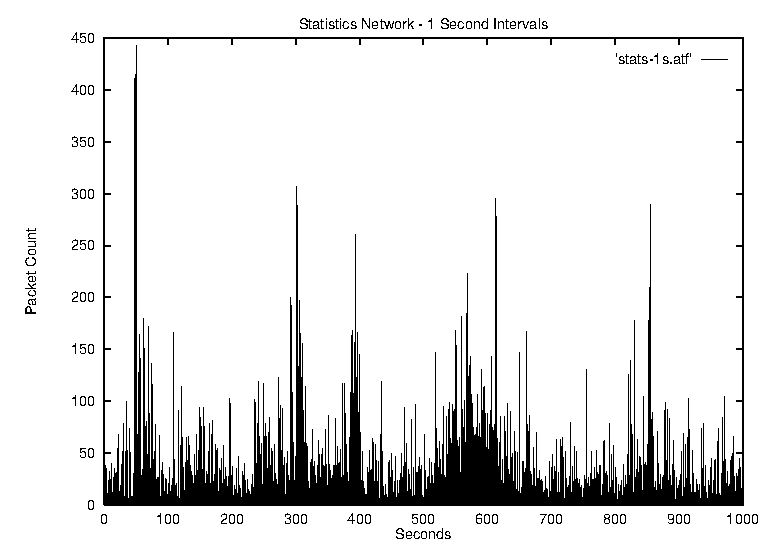
\includegraphics[height=3in]{pics/snet93-1s-freq.eps}
\caption{Statistics network with time interval 1 second}
\label{results:snet93.1s.freq}
\end{figure}

\begin{figure}
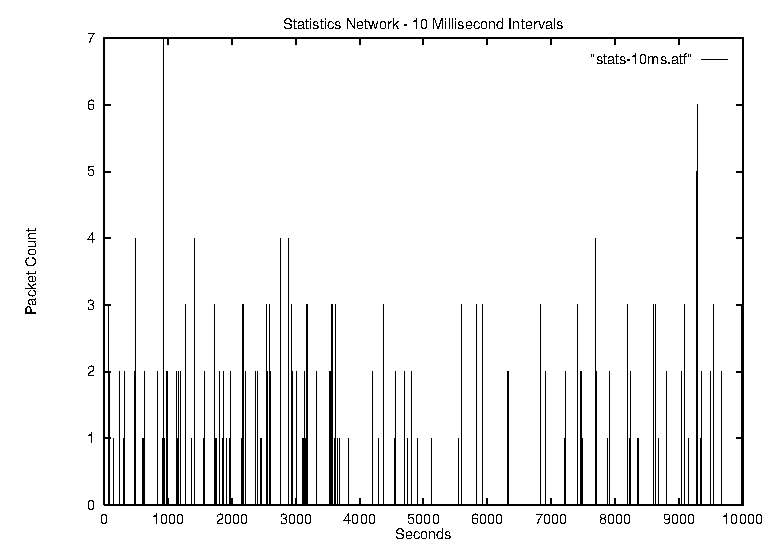
\includegraphics[height=3in]{pics/snet93-10ms-freq.eps}
\caption{Statistics network with time interval 10 milliseconds}
\label{results:snet93.10ms.freq}
\end{figure}

\begin{figure}
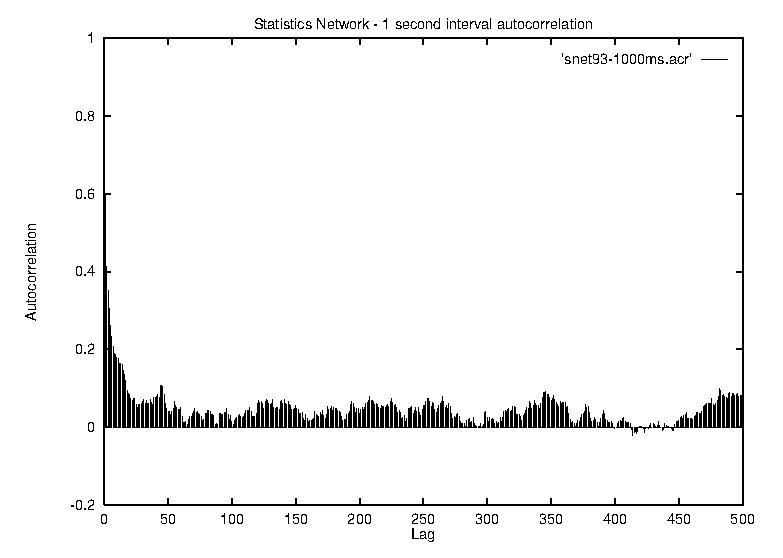
\includegraphics[height=3in]{pics/snet93-1s-acr.eps}
\caption{Statistics network autocorrelation with time interval 1 second}
\label{results:snet93.1s.acr}
\end{figure}

\begin{figure}
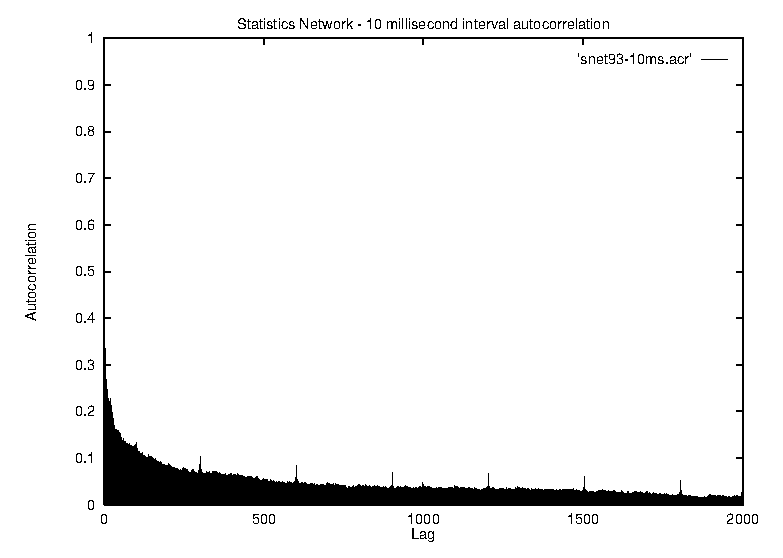
\includegraphics[height=3in]{pics/snet93-10ms-acr.eps}
\caption{Statistics network autocorrelation with time interval 10 milliseconds}
\label{results:snet93.10ms.acr}
\end{figure}

\begin{figure}
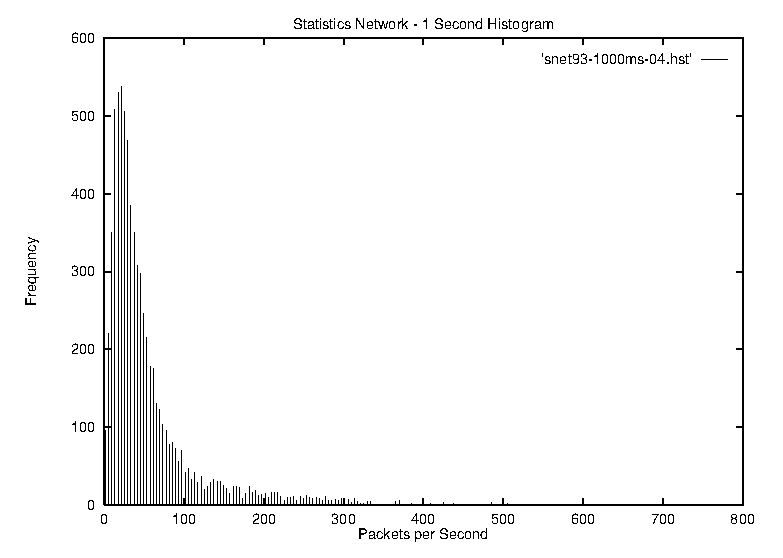
\includegraphics[height=3in]{pics/snet93-1s-hist-04.eps}
\caption{Statistics network histogram with time interval 1 second}
\label{results:snet93.1s.hist}
\end{figure}

The Department of Statistics staff subnetwork (also known as subnet
93) consists of about twenty Sun workstations using NIS and NFS
and some Macintoshes.  Apart from file and print server traffic it
also carries some X-windows traffic.

Figure~\ref{results:snet93.1s.freq} shows a much more lightly loaded
segment with minimal background traffic but still exhibiting very
bursty traffic.  The 10 millisecond autocorrelation
(figure~\ref{results:snet93.10ms.acr}) shows definite peaks every 300
milliseconds.  This is caused by the router broadcasting IP routeing
information.  It is not a very large amount of information (about
seven small sized packets sent back to back) indicating that the level
of background traffic is small (since it does not mask the route
broadcasts).  The histogram (figure ~\ref{results:snet93.1s.hist})
shows most of the traffic flows at a steady level and that bursts are
low in number and size.

\subsubsection{External gateway network of the University}

\begin{figure}
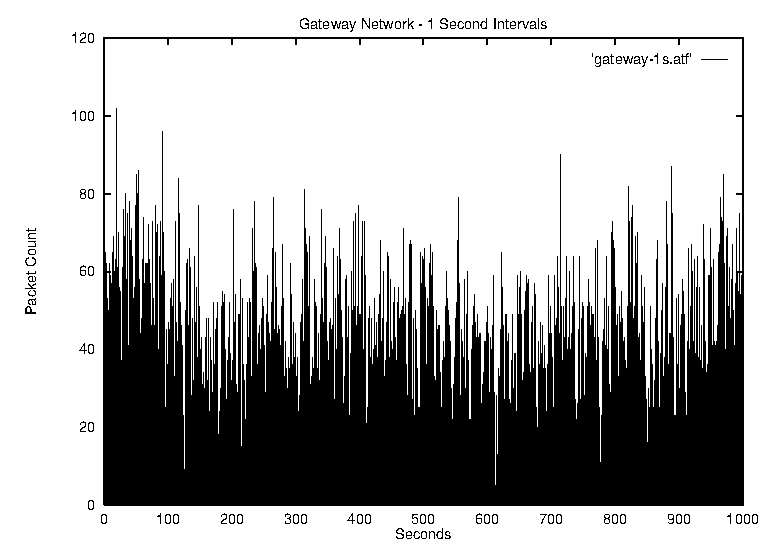
\includegraphics[height=3in]{pics/gatew-1s-freq.eps}
\caption{Gateway network with time interval 1 second}
\label{results:gatew.1s.freq}
\end{figure}

\begin{figure}
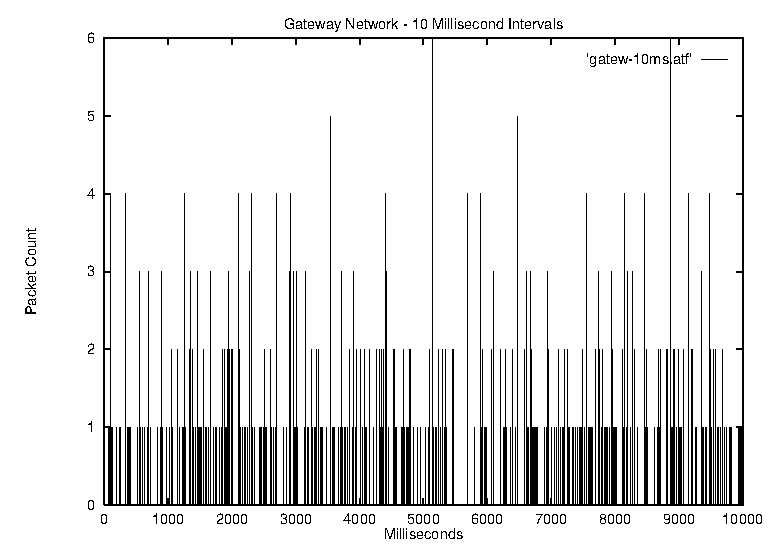
\includegraphics[height=3in]{pics/gatew-10ms-freq.eps}
\caption{Gateway network with time interval 10 millisecond}
\label{results:gatew.10ms.freq}
\end{figure}

\begin{figure}
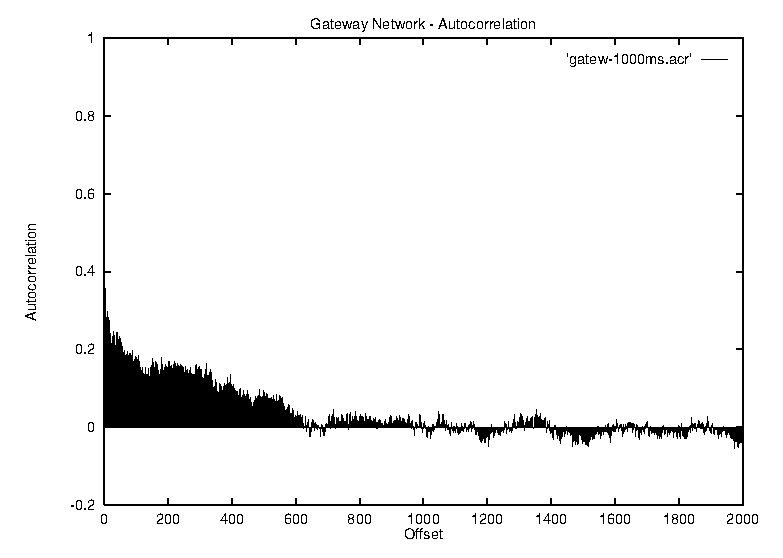
\includegraphics[height=3in]{pics/gatew-1s-acr.eps}
\caption{Gateway network autocorrelation with time interval 1 second}
\label{results:gatew.1s.acr}
\end{figure}

\begin{figure}
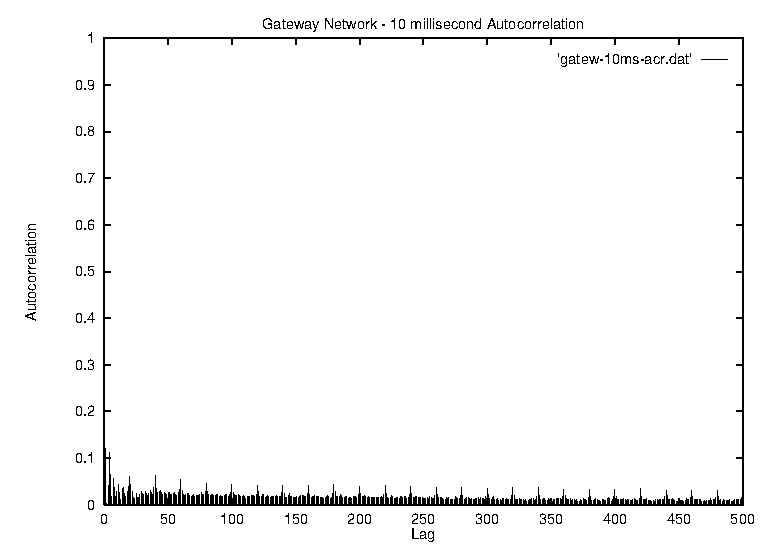
\includegraphics[height=3in]{pics/gatew-10ms-acr.eps}
\caption{Gateway network autocorrelation with time interval 10 milliseconds}
\label{results:gatew.10ms.acr}
\end{figure}

\begin{figure}
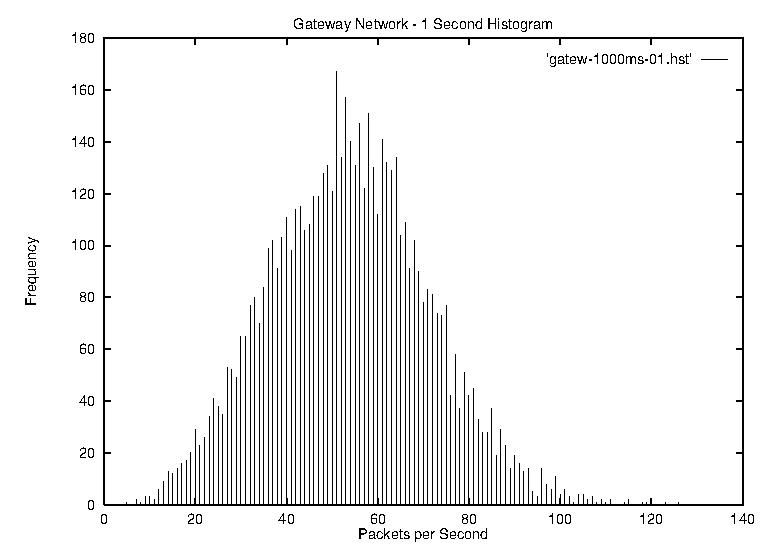
\includegraphics[height=3in]{pics/gatew-1s-hist-01.eps}
\caption{Gateway network histogram with time interval 1 second}
\label{results:gatew.1s.hist}
\end{figure}

The Gateway Network (figure~\ref{results:gatew.1s.freq}) has an
extremely light load with a considerable amount (with respect to the
total) of the traffic as a steady background flow.  The bursts are
much smaller in comparison to the other segments, with virtually all
the traffic consisting of TCP/IP.  The 1 second autocorrelation
(figure
\ref{results:gatew.1s.acr}) shows that there exists a dependency that
decays steadily with lag until it becomes noise around the 10 minute
lag time.  The 10 millisecond autocorrelation (figure
\ref{results:gatew.10ms.acr}) shows periodic behaviour every 200
milliseconds.  I am uncertain as to its exact cause but it could well
be Network Time Protocol (NTP) \cite{RFC:1305}.

The histogram (figure \ref{results:gatew.1s.hist}) shows very steady
traffic flows without any large bursts.  This link is connected to a
128 kbit connection to the outside world so the size of bursts would
be limited in any case but the unimodal, approximately symmetric shape
of the histogram most likely comes from the steady flow of USENET
traffic and the congestion control used by TCP.

\subsubsection{Commerce postgraduate teaching laboratory}

\begin{figure}
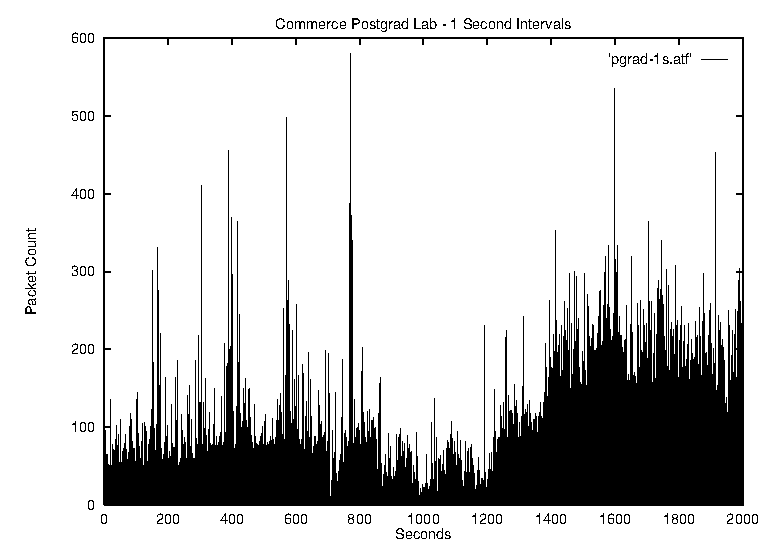
\includegraphics[height=3in]{pics/pgrad-1s-freq.eps}
\caption{Commerce Postgraduate Lab with time interval 1 second}
\label{results:pgrad.1s.freq}
\end{figure}


\begin{figure}
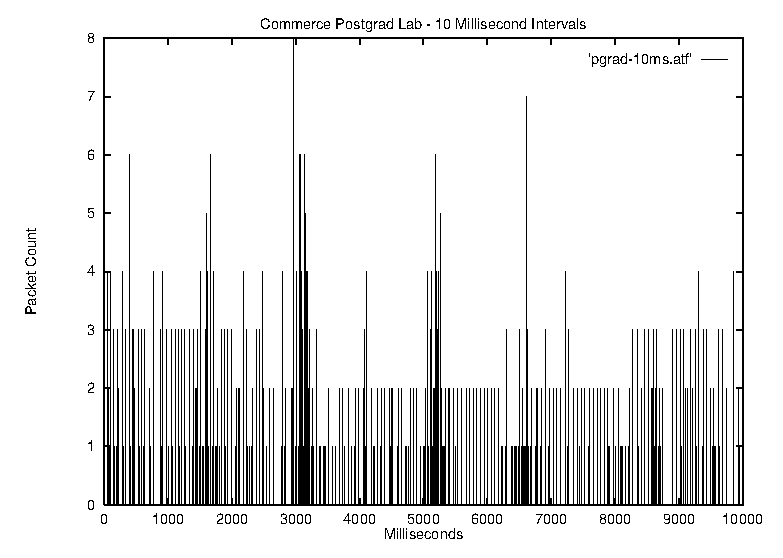
\includegraphics[height=3in]{pics/pgrad-10ms-freq.eps}
\caption{Commerce Postgraduate Lab with time interval 10 milliseconds}
\label{results:pgrad.10ms.freq}
\end{figure}

\begin{figure}
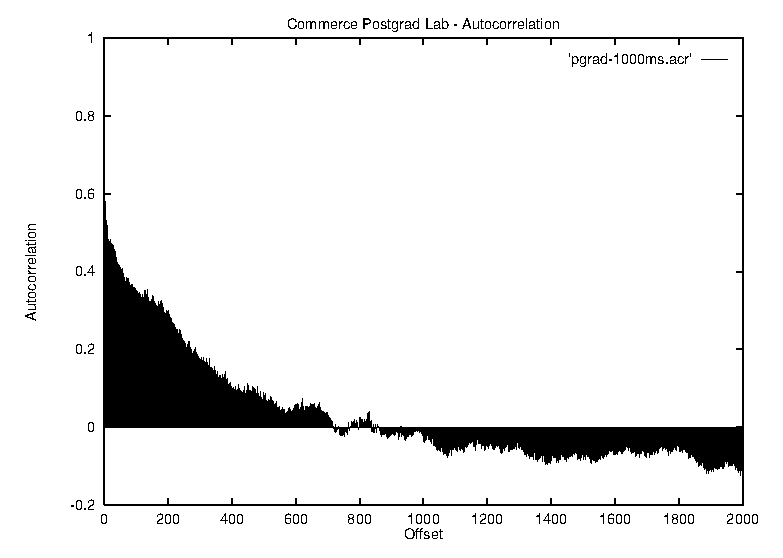
\includegraphics[height=3in]{pics/pgrad-1s-acr.eps}
\caption{Commerce Postgraduate Lab autocorrelation with time interval 1 second}
\label{results:pgrad.1s.acr}
\end{figure}

\begin{figure}
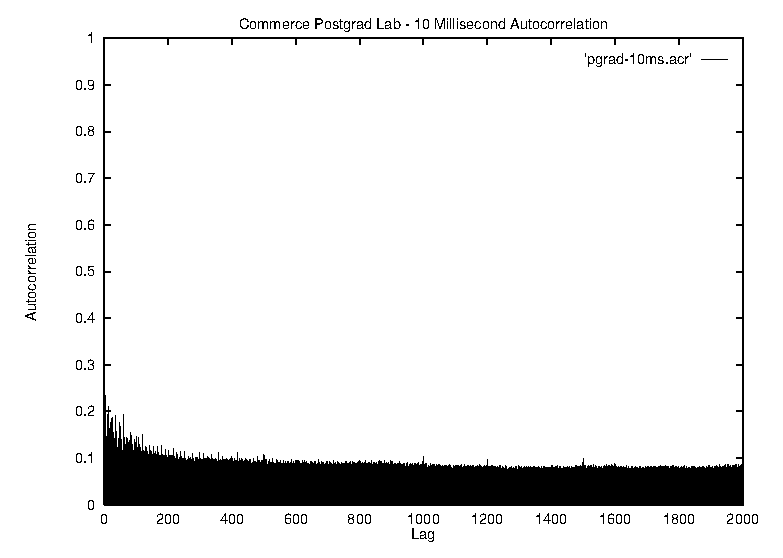
\includegraphics[height=3in]{pics/pgrad-10ms-acr.eps}
\caption{Commerce Postgraduate Lab autocorrelation with time interval 10 milliseconds}
\label{results:pgrad.10ms.acr}
\end{figure}

\begin{figure}
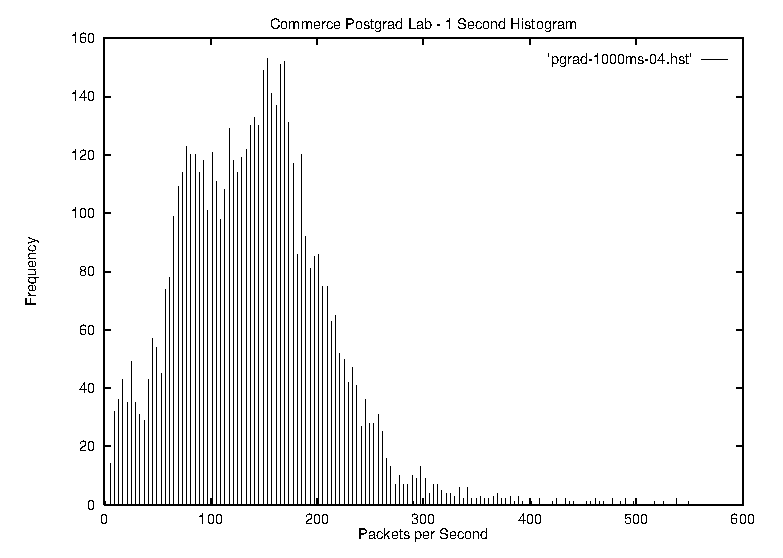
\includegraphics[height=3in]{pics/pgrad-1s-hist-04.eps}
\caption{Commerce Postgraduate histogram Lab with time interval 1 second}
\label{results:pgrad.1s.hist}
\end{figure}

The Commerce Postgraduate teaching laboratory consists of about twenty
personal computers running Windows For Workgroups.  They connect to a
Windows NT server using the NetBIOS LAN protocol.

This segment has a reasonably heavy load and only has NetBIOS traffic.
The down loading of large windows applications (over two megabytes or
more) creates large bursts of traffic.

NetBIOS has no routeing information and no directory system so there
is minimal periodic background traffic.  The figures
\ref{results:pgrad.1s.freq} and \ref{results:pgrad.10ms.freq} show a
steady level of traffic with only a few notable peaks.  This behaviour
is echoed in the histogram (figure \ref{results:pgrad.1s.hist})
showing that most of the traffic occured as steady flows.

\subsection{Graphs by protocol}

Below are three graphs showing the most prevalent protocols used
around the university, that is IP (\S \ref{network:ip}, AppleTalk (\S 
\ref{network:appletalk}) and Netware IPX (\S \ref{network:ipx}).

\subsubsection{Internet Protocol}

\begin{figure}
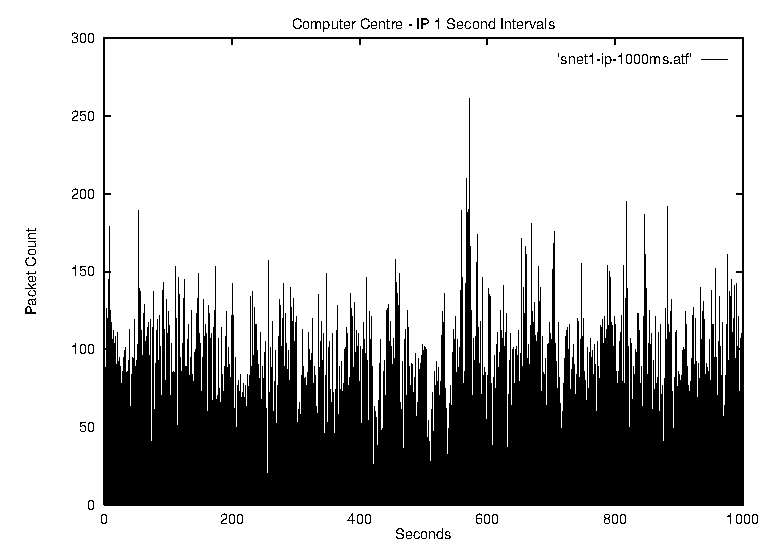
\includegraphics[height=3in]{pics/snet1-ip-1s-freq.eps}
\caption{IP traffic on Computer Centre network with time interval 1 second}
\label{results:snet1.ip.1s.freq}
\end{figure}

\begin{figure}
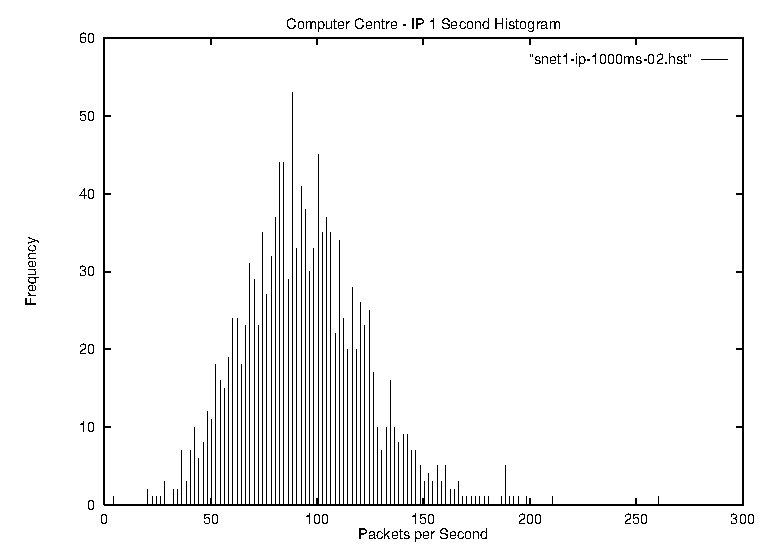
\includegraphics[height=3in]{pics/snet1-ip-1s-hist-02.eps}
\caption{Histogram of IP traffic on Computer Centre network with time interval 1 second}
\label{results:snet1.ip.1s.hist}
\end{figure}


Figure~\ref{results:snet1.ip.1s.freq} shows Internet Protocols traffic.
This graph shows a reasonable (with respect to the peak maximums)
amount of background traffic.  This is most likely a result of a
steady level of remote login and mail traffic.

\subsubsection{AppleTalk}

\begin{figure}
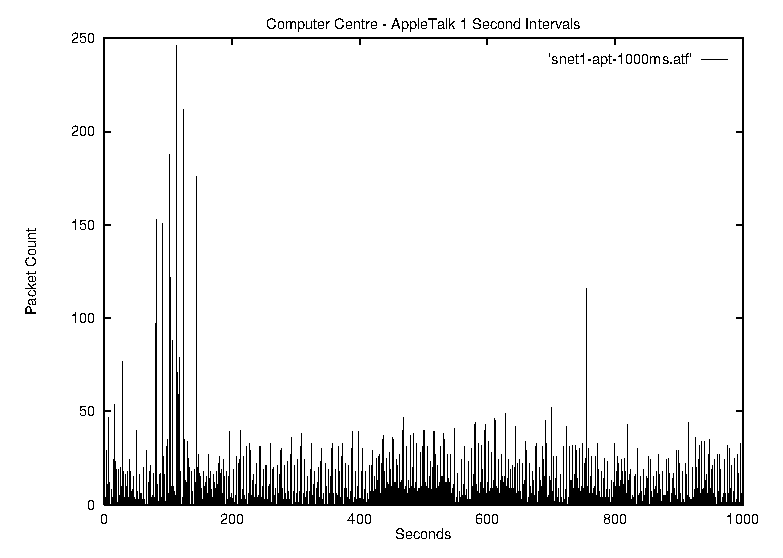
\includegraphics[height=3in]{pics/snet1-apt-1s-freq.eps}
\caption{AppleTalk traffic on Computer Centre network with time interval 1 second}
\label{results:snet1.apt.1s.freq}
\end{figure}

\begin{figure}
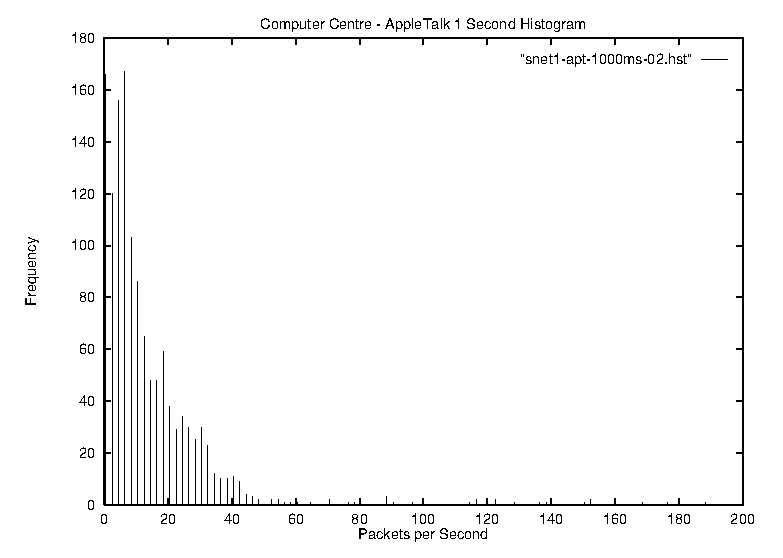
\includegraphics[height=3in]{pics/snet1-apt-1s-hist-02.eps}
\caption{Histogram of AppleTalk traffic on Computer Centre network with time interval 1 second}
\label{results:snet1.apt.1s.hist}
\end{figure}

Figure~\ref{results:snet1.apt.1s.freq} shows AppleTalk traffic on the
Computer Centre network.  Because there is very little AppleTalk
traffic on subnet 1 events become more pronounced and noticeable.
AppleTalk has periodic broadcasts to relay routeing and directory
services (zone maps) information.

\subsubsection{Netware IPX}

\begin{figure}
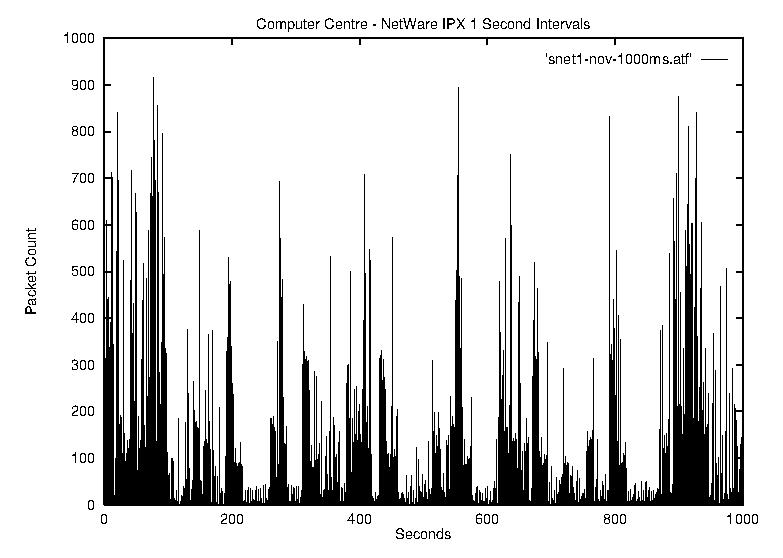
\includegraphics[height=3in]{pics/snet1-ipx-1s-freq.eps}
\caption{IPX traffic on Computer Centre network with time interval 1 second}
\label{results:snet1.nov.1s.freq}
\end{figure}

\begin{figure}
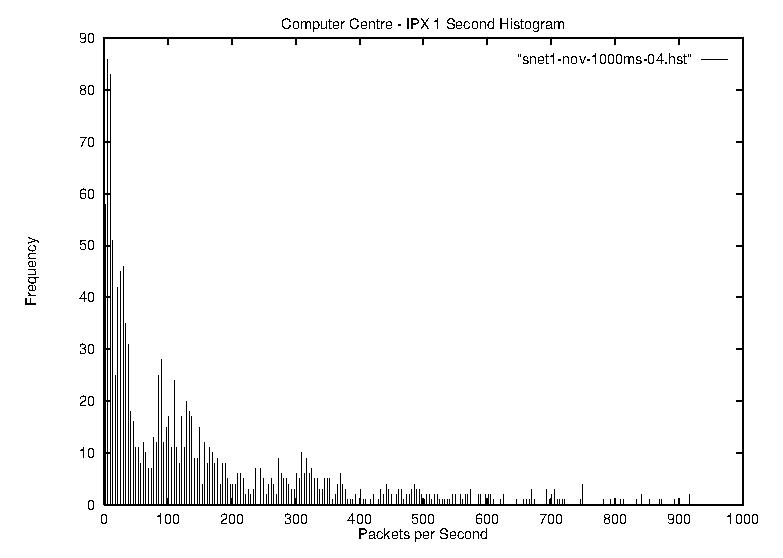
\includegraphics[height=3in]{pics/snet1-ipx-1s-hist-02.eps}
\caption{Histogram of IPX traffic on Computer Centre network with time interval 1 second}
\label{results:snet1.nov.1s.hist}
\end{figure}

\begin{figure}
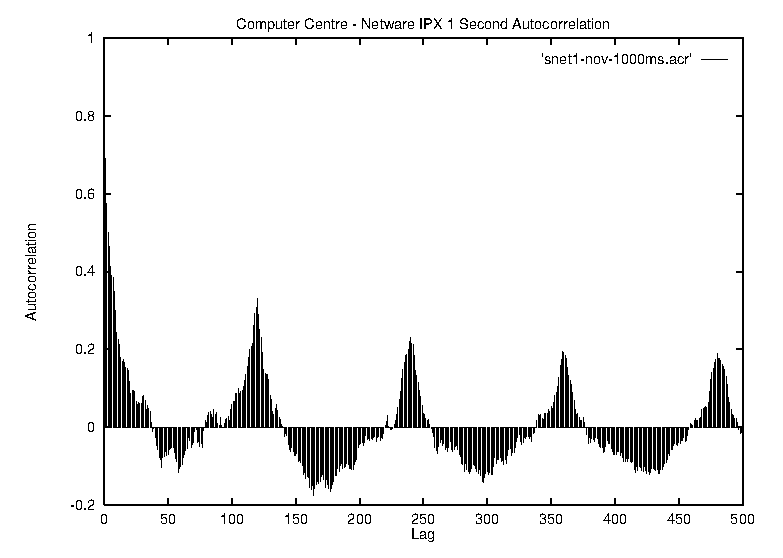
\includegraphics[height=3in]{pics/snet1-ipx-1s-acr.eps}
\caption{Autocorrelation of IPX traffic on Computer Centre network with time interval 1 second}
\label{results:snet1.nov.1s.acr}
\end{figure}

Figure~\ref{results:snet1.nov.1s.freq} show Netware traffic on the
Computer Centre network.  While it looks as though there is
considerable IPX traffic in fact there is little file transfer
traffic.  The large bursts of traffic come from Netware's service
announcements.  Every two minutes Netware capable routers broadcast
all available Netware services, such as file servers, printing
spoolers and mail exchanges.  Due to the number of these services
around the university it amounts to over 500 kilobytes of information.
This is clearly seen in the autocorrelation (figure
\ref{results:snet1.nov.1s.acr}).

\clearpage

\section{Slowly decaying variance}

Figures \ref{results:snet1.10ms.sta}, \ref{results:gatew.10ms.sta},
\ref{results:snet93.10ms.sta} and \ref{results:pgrad.10ms.sta} all
show the slowly decaying variance associated with self-similar
behaviour.  The plots are created from the output of \texttt{stat}
program (\S \ref{results:stat}.  The plots use the logarithm base 10
output from \texttt{stat}.  This is the same as the slowly decaying
variance plots in the Bellcore papers \cite{Bell:1} \cite{Bell:2}.
Each plot includes a line with slope $y = -x$ for reference (the
theoretical slope for a general renewal is $y = x^{-1}$, so taking the
logarithm gives $y = -x$).  While each plot is unique they all have a
similar shape and clearly show slowly decaying behaviour.

While is obvious that the shapes are different, because of the
differences in the samples there is no simple explanation as to how the
shape of the curve relates to the underlying traffic behaviour.

\begin{figure}
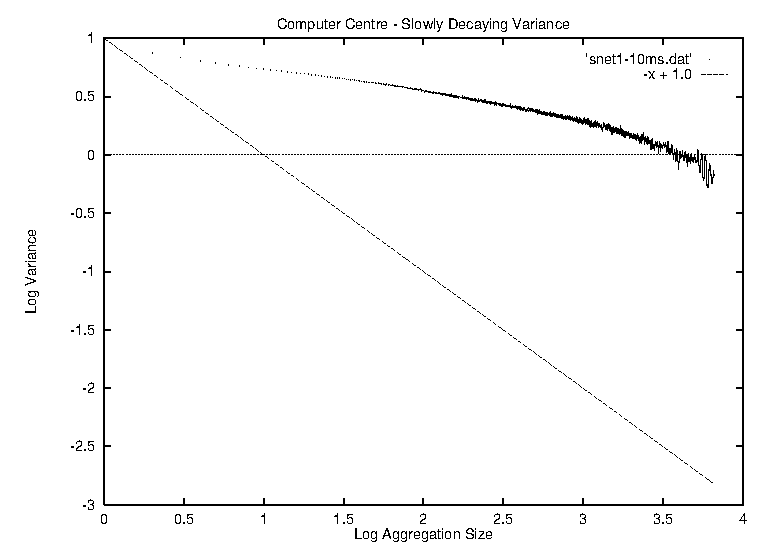
\includegraphics[height=3in]{pics/snet1-10ms-sta.eps}
\caption{Slowly decaying variance plot of the Computer Centre network}
\label{results:snet1.10ms.sta}
\end{figure}

\begin{figure}
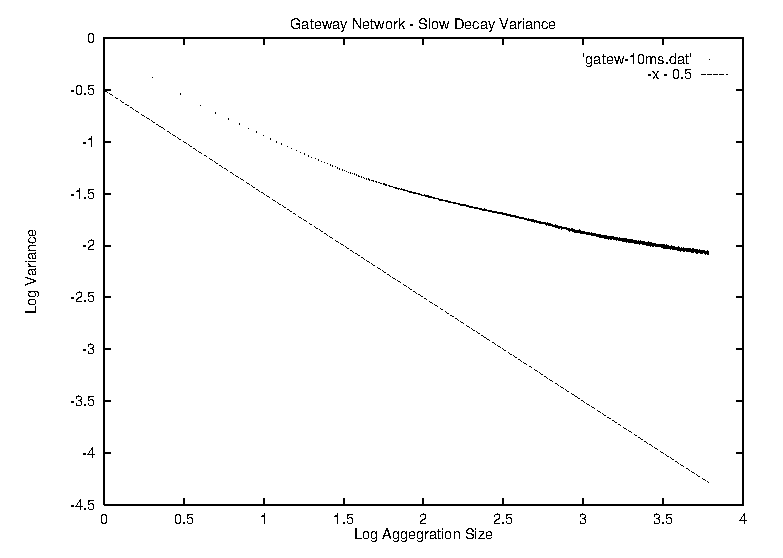
\includegraphics[height=3in]{pics/gatew-10ms-sta.eps}
\caption{Slowly decaying variance plot of the Gateway network}
\label{results:gatew.10ms.sta}
\end{figure}

\begin{figure}
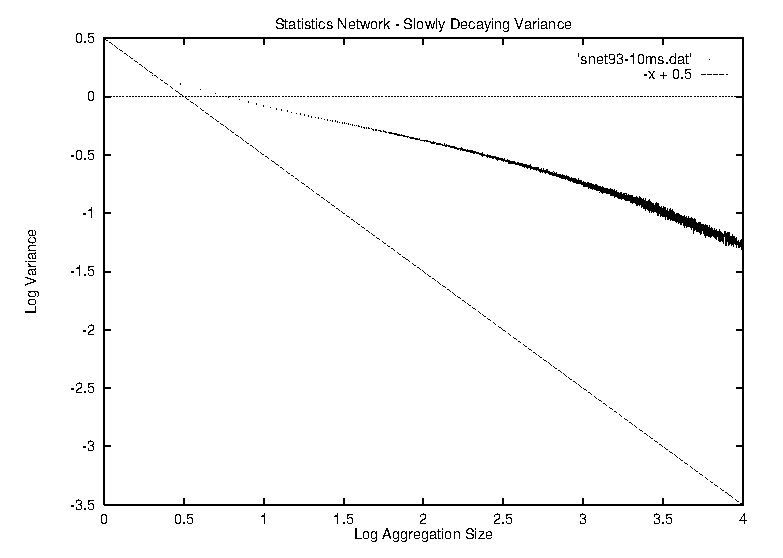
\includegraphics[height=3in]{pics/snet93-10ms-sta.eps}
\caption{Slowly decaying variance plot of the Statistics network}
\label{results:snet93.10ms.sta}
\end{figure}

\begin{figure}
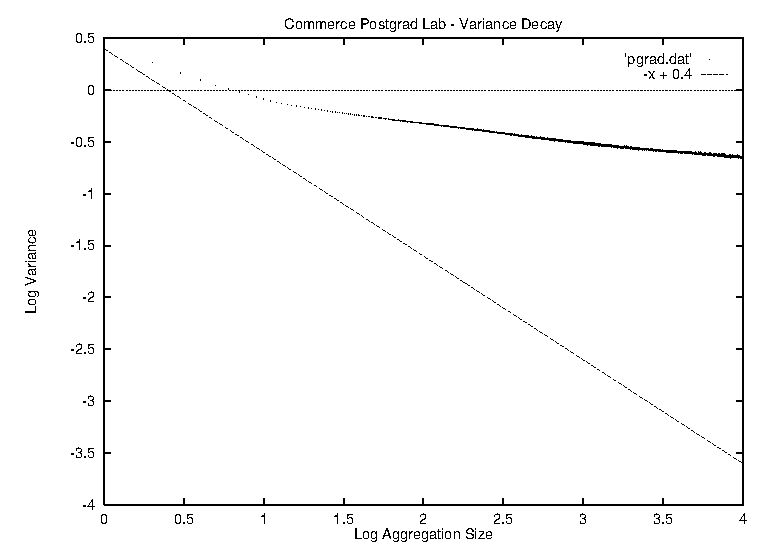
\includegraphics[height=3in]{pics/pgrad-10ms-sta.eps}
\caption{Slowly decaying variance plot of the Commerce Postgraduate network}
\label{results:pgrad.10ms.sta}
\end{figure}

